\section{Software Guard Extensions (SGX)}
\label{sec:sgx}

This section summarizes the aspects of the SGX documentation that are relevant
to our system. The interested but time-constrained reader is advised to read
\cite{mckeen2013innovative}, \cite{anati2013sgx}, and Chapters 1 (Introduction
to SGX), 3 (Enclave Operation), 4 (Enclave Exiting Events) and 6 (SGX
Interactions with IA32 and Intel 64 Architecture) of \cite{intel2013sgxmanual}
for a deeper understanding of SGX.


\subsection{SGX Overview}
\label{sec:sgx_overview}

SGX introduces a protected execution environment, called an \textit{enclave}.
An enclave's code and data are protected by placing them inside the Enclave
Page Cache (EPC), which is a subset of the Processor Reserved Memory (PRM)
area. The EPC is split in 4KB pages. Each page is associated with an enclave.
EPC page memory accesses coming from code outside the EPC page's enclave are
blocked by the CPU. This access check covers all privilege levels, including
SMM. The memory controller inside the CPU blocks any DMA access to PRM, so EPC
pages cannot be accessed by hardware via DMA.

The EPC contents is encrypted\footnote{Actually, the SGX manual carefully
tiptoes around this issue by saying ``On implementations in which EPC is part
of system DRAM, the contents of the EPC are protected by an encryption
engine.''} as it leaves the CPU, to prevent against bus tapping attacks.
Although the data is encrypted, the memory addresses are not protected,
exposing the enclave code's memory access patterns.

Execution flow can only enter an enclave via special CPU instructions
(\texttt{EENTER}, \texttt{ERESUME}, \texttt{EEXIT}), which are similar to the
mechanism for switching from user mode to kernel mode. Enclave execution always
happens in protected mode, at ring 3, and uses the address translation set up
by the OS kernel and hypervisor (\S \ref{sec:paging}). \texttt{EENTER}
transfers control to a predefined entry point in the enclave, and
\texttt{EEXIT} leaves the enclave.

To avoid leaking private data, a CPU that is executing enclave code does not
directly service an interrupt, fault (e.g., a page fault) or VM exit. Instead,
the CPU first performs an Asynchronous Enclave Exit (AEX) to switch from
enclave code to ring 3 code, and then services the interrupt, fault, or VM
exit.  The CPU performs an AEX by saving the CPU state into a predefined area
inside the enclave and transfers control to a pre-specified instruction outside
the enclave, replacing CPU registers with synthetic values. After the
interrupt, fault or VM exit is serviced, its handler returns control to ring 3
code outside the enclave, which performs an \texttt{ERESUME}, which transfers
control back into the enclave and restores the CPU state at the time the
enclave execution was interrupted.

The allocation of EPC pages to enclaves is delegated to the OS kernel (or
hypervisor), and done via dedicated ring 0 CPU instructions. \texttt{EADD}
allocates new pages to an enclave under construction, and \texttt{EREMOVE}
deallocates pages during enclave tear-down. \texttt{EWB} evicts\footnote{
Multi-threaded enclaves require more steps that are orthogonal to the issues
addressed by this work.} an EPC page to RAM space that the OS kernel can
access, and \texttt{ELDB}\footnote{SGX specifies two related instructions,
\texttt{ELDB} and \texttt{ELDU}. The distinction is irrelevant for our
purposes.} loads a previously evicted page from kernel-acessible RAM back into
the EPC.

\texttt{EADD} associates each EPC page with a virtual address used to access
it, and the association is maintained by the \texttt{EWB} / \texttt{ELDB} pair.
The CPU enforces\footnote{The CPU generates a general protection fault (\#GP)
if an address translation that results in an EPC page uses the wrong virtual
address as input.} the invariant that an EPC page can only be accessed using
the virtual address associated with it. This mechanism ensures that the OS
kernel and hypervisor maintain a consistent mapping of virtual addresses to
EPC pages. The CPU encrypts and HMACs pages evicted with \texttt{EWB},
providing privacy and integrity guarantees, including protection against replay
attacks. The details are described in \cite{intel2013sgxmanual}.

Page faults in enclave code are handled using the AEX process. The CR2
register, which normally holds the virtual address that causes the fault, has
its bottom 12 bits set to zero. The other bits of CR2 are necessary for the OS
kernel or hypervisor to know which page needs to be loaded in RAM or into the
EPC. This allows a curious OS kernel or hypervisor to obtain a page-level
memory access trace for a program running inside an enclave, simply by making
sure that only one page is present at any given time.


\subsection{SGX Information Leaks}
\label{sec:sgx_leaks}

Software Guard Extensions, as documented in \cite{intel2013sgxmanual}, does not
provide full privacy guarantees to the code executing inside an enclave. We
present methods that an attacker can use to extract information from an
enclave.

\subsubsection{Hyper-Threading Leaks}

Modern Intel CPUs feature hyper-threading, which means that each core has two
(or more) sets of register files and local APICs, presented as logical
processors running separate threads (see Figure \ref{fig:cpu_core}). The
threads share the other core resources, such as the fetch and decode units,
execution units and L1 and L2 caches. SGX does not prevent hyper-threading, so
a malicious OS kernel or hypervisor can schedule a thread executing enclave
code and a snooping thread on logical processors on same core. The snooping
thread can use the processor's high-performance counter
\cite{petters1999making} to get information about the instructions and memory
access patterns of the thread executing enclave code.

\begin{figure}[hbtp]
  \center{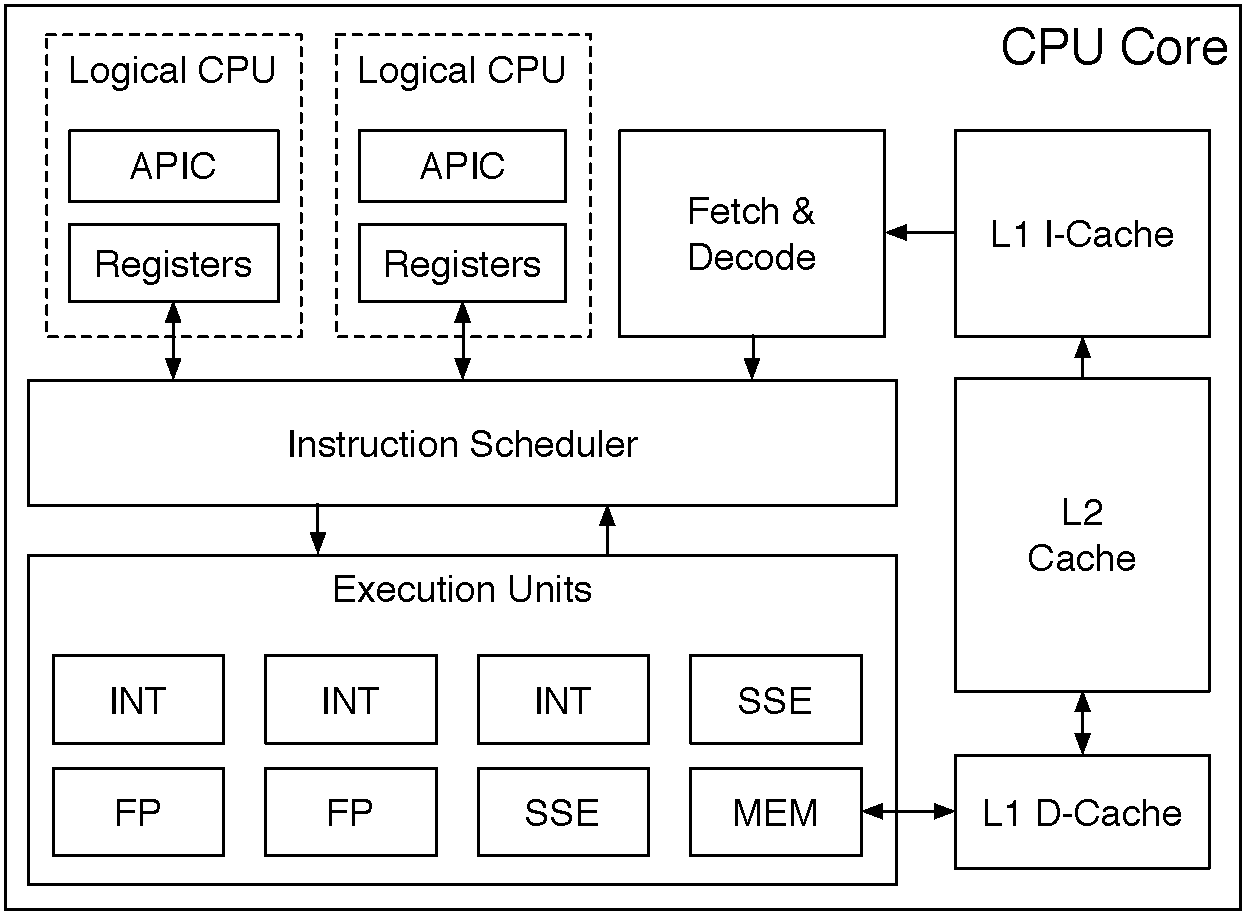
\includegraphics[width=85mm]{figures/cpu_core.pdf}}
  \caption{
    CPU core with two logical processors. Each logical processor has its own
    APIC and execution state, and they share all the other core resources.
  }
  \label{fig:cpu_core}
\end{figure}

A promising approach for preventing against hyper-threading leaks is to
effectively disable hyper-threading, by using \texttt{CPUID} to find out the
number of logical processors in the current core, and to require the OS to
schedule threads in the same enclave on all the logical processors. This could
be implemented by having the main thread spinlock waiting for the other threads
to start, before any protected computation is performed. However, a malicious
kernel or hypervisor can de-schedule the other threads after the main thread
performed the spinlock check, so this defense is not reliable.

\subsubsection{Page-Level Memory Access Leaks}

While executing the code inside an enclave, the CPU still follows the standard
page translation process (\S \ref{sec:paging}), including setting the A and D
bits and delivering page faults. A malicious OS kernel or hypervisor can
obtain the page-level trace of an application executing inside an enclave by
setting the P flag to 0 on all the enclave's pages before starting enclave
execution, and then maintaining exactly one instruction page and one data page
present in the enclave's address space.

When a page fault is generated, CR2 contains the virtual address of a page
accessed by enclave, and the error code indicates whether the memory access was
a read or a write (bit 1) and whether the memory access is a data access or
an instruction fetch access (bit 4). On a data access, the kernel tracing the
enclave code's memory access pattern would set the P flag of the desired page
to 1, and set the P flag of the previously accessed data page to 0. Instruction
accesses can be handled in a similar manner.

For a slightly more detailed trace, the kernel can set a desired page's W flag
to 0 if the page fault's error code indicates a read access, and only set it to
1 for write accesses. Also, applications that use a page as both code and data
(self-modifying code and just-in-time compiling VMs) can be handled by setting
a page's XD flag to 0 for a data access, and by carefully accounting for the
case where the last accessed data page is the same as the last accessed code
page.

Leaving an enclave via an AEX and re-entering the enclave via \texttt{ERESUME}
causes the CPU to flush TLB entries that contain enclave addresses, so a
tracing kernel would not need to worry about flushing the TLB. The tracing
kernel does not need to flush the caches either, because the CPU needs to
perform address translation even for cached data.

An easy way to reduce this attack's power is to increase the page size, so the
trace contains less information. However, the attack cannot be completely
prevented without removing the kernel's ability to oversubscribe the EPC,
which is a major benefit of paging.

\subsubsection{Fine-Grained Memory Access Leaks}

The AEX process and the \texttt{ERESUME} instructions do not flush the CPU
caches. A tracing kernel can take advantage of cache timing to narrow down
the addresses in an application's memory access trace to cache line
granularity, by extending the method described above with the steps below.

The tracing kernel controls the mapping between virtual addresses and physical
addresses, so it can make sure that its own code and data use different sets
in the L2 cache from the enclave's code and data. For example, in a typical
256kb (per-core) L2 cache organized as 512 8-way sets of 64-byte lines, the
tracing kernel could allocate lines 0-63 for the enclave's code page, lines
64-127 for the enclave's data page, and use lines 128-511 for its own pages.

Right before entering an enclave via \texttt{EENTER} or \texttt{ERESUME}, the
kernel would issue \texttt{CLFLUSH} instructions to flush the enclave's code
page and data page from the cache. The enclave could have accessed a single
code page and a single data pages, so flushing the cache should be reasonably
efficient. The tracing kernel then uses 16 bogus pages (8 for the enclave's
code page, and 8 for the enclave's data page) to load all the 8 ways in the 128
cache sets allocated by enclave pages. After an AEX gives control back to the
tracing kernel, it can read the 16 bogus pages, and exploit the time difference
between an L2 cache hit and a miss to see which cache lines were evicted and
replaced by the enclave's memory accesses.

\subsubsection{Leaks via Physical Attacks}

The methods described above rely on a compromised hypervisor or OS kernel, but
not on physical attacks. If an attacker can tap into the memory bus and read
the address lines, the attacker can learn the enclave code's memory access
patterns, at a fine granularity.

The processor reserved memory (PRM) is configured by the BIOS at boot time as
a continuous memory area, and can be configured as write-back (WB) or
uncacheable (UC) memory. If the PRM is uncacheable, the CPU will generate a
memory transaction for every memory access. The granularity of the memory
transactions depends on the encryption engine used for the EPC, which is not
documented in \cite{intel2013sgxmanual}. If 128-bit AES is used, memory tapping
would yield addresses at 16-byte granularity, which means two 64-bit words.

At the same time, configuring the PRM as uncacheable memory removes the cache
timing attack documented above, at the cost of dramatically slowing down the
execution of SGX code. In this case, the CPU would still leak memory access
patterns at page granularity, due to the address translation engine.
